\begin{enumerate}[label=\thesection.\arabic*,ref=\thesection.\theenumi]
\item  Show that the three lines with direction cosines
$\frac{12}{13},\frac{-3}{13},\frac{-4}{13}$; $\frac{4}{13},\frac{12}{13},\frac{3}{13}$; $\frac{3}{13},\frac{-4}{13},\frac{12}{13}$; are mutually perpendicular.\\
    \solution
		\iffalse
\documentclass[12pt]{article}
\usepackage{graphicx}
\usepackage{amsmath}
\usepackage{mathtools}
\usepackage{gensymb}
\usepackage[utf8]{inputenc}
\usepackage{float}
\usepackage{setspace}
\newcommand{\mydet}[1]{\ensuremath{\begin{vmatrix}#1\end{vmatrix}}}
\providecommand{\brak}[1]{\ensuremath{\left(#1\right)}}
\providecommand{\norm}[1]{\left\lVert#1\right\rVert}
\newcommand{\solution}{\noindent \textbf{Solution: }}
\newcommand{\myvec}[1]{\ensuremath{\begin{pmatrix}#1\end{pmatrix}}}
\let\vec\mathbf

\begin{document}
\begin{center}
\textbf\large{CLASS-12 \\ CHAPTER-11 \\ THREE DIMENSIONAL GEOMETRY}
\end{center}
\section*{Excercise 11.2}

Q1. Show that the three lines with direction cosines $\frac{12}{13}, \frac{-3}{13}, \frac{-4}{13}; \frac{4}{13}, \frac{12}{13}, \frac{3}{13}; \frac{3}{13}, \frac{-4}{13}, \frac{12}{13}$ are mutually perpendicular.
\\
\solution
\fi
Let
	\begin{align}
			\vec{A}=\myvec{\frac{12}{13}\\[2pt]\frac{-3}{13}\\[2pt]\frac{-4}{13}},\vec{B}=\myvec{\frac{4}{13}\\[2pt]\frac{12}{13}\\[2pt]\frac{3}{13}},\vec{C}=\myvec{\frac{3}{13}\\[2pt]\frac{-4}{13}\\[2pt]\frac{12}{13}}
		\end{align}
		Stacking all three vectors into a single matrix 
			\begin{align}
		\vec{P}=\myvec{\frac{12}{13}&\frac{4}{13}    &\frac{3}{13}\\[2pt] \frac{-3}{13}&\frac{12}{13}&\frac{-4}{13}\\[2pt] \frac{-4}{13}&\frac{3}{13}&\frac{12}{13}}, \vec{P}^\top=\myvec{\frac{12}{13}&\frac{-3}{13}   &\frac{-4}{13}\\[2pt] \frac{4}{13}&\frac{12}{13}&\frac{3}{13}\\[2pt] \frac{3}{13}&\frac{-4}{13}&\frac{12}{13}},
			\end{align}
			we obtain
			\begin{align}
		\vec{P}\vec{P}^\top=
				\myvec{\frac{12}{13}&\frac{4}{13}    &\frac{3}{13}\\[2pt] \frac{-3}{13}&\frac{12}{13}&\frac{-4}{13}\\[2pt] \frac{-4}{13}&\frac{3}{13}&\frac{12}{13}}\myvec{\frac{12}{13}&\frac{-3}{13}   &\frac{-4}{13}\\[2pt] \frac{4}{13}&\frac{12}{13}&\frac{3}{13}\\[2pt] \frac{3}{13}&\frac{-4}{13}&\frac{12}{13}}=\vec{I} =
	\vec{P}^\top\vec{P}
		\end{align}
					Hence, all three vectors are orthogonal to each other.




\item  Show that the line through the points $(1,-1,2),(3,4,-2 )$ is perpendicular to the line through the points$(0,3,2)$ and$(3,5,6)$.\\
    \solution
		\iffalse
\documentclass[12pt]{article}
\usepackage{graphicx}
\usepackage[none]{hyphenat}
\usepackage{graphicx}
\usepackage{listings}
\usepackage[english]{babel}
\usepackage{graphicx}
\usepackage{caption} 
\usepackage{booktabs}
\usepackage{array}
\usepackage{amssymb} % for \because
\usepackage{amsmath}   % for having text in math mode
\usepackage{extarrows} % for Row operations arrows
\usepackage{listings}
\lstset{
  frame=single,
  breaklines=true
}
\usepackage{hyperref}
  
%Following 2 lines were added to remove the blank page at the beginning
\usepackage{atbegshi}% http://ctan.org/pkg/atbegshi
\AtBeginDocument{\AtBeginShipoutNext{\AtBeginShipoutDiscard}}


%New macro definitions
\newcommand{\mydet}[1]{\ensuremath{\begin{vmatrix}#1\end{vmatrix}}}
\providecommand{\brak}[1]{\ensuremath{\left(#1\right)}}
\providecommand{\norm}[1]{\left\lVert#1\right\rVert}
\newcommand{\solution}{\noindent \textbf{Solution: }}
\newcommand{\myvec}[1]{\ensuremath{\begin{pmatrix}#1\end{pmatrix}}}
\providecommand{\abs}[1]{\left\vert#1\right\vert}
\let\vec\mathbf

\begin{document}

\begin{center}
\title{\textbf{Equation  of Perpendicular}}
\date{\vspace{-5ex}} %Not to print date automatically
\maketitle
\end{center}
\setcounter{page}{1}
\section{12$^{th}$ Maths - Chapter 11}
\textbf{This is Problem-2 from Exercise 11.2}
\begin{enumerate}
\item Show that the line through the points (1, -1, 2), (3, 4, -2) is perpendicular to the line through the points (0, 3, 2) and (3, 5, 6).
\item \textbf{Solution :}
	\fi
	Let
\begin{align}  
\vec{A}=\myvec{1 \\-1\\2},\,
\vec{B}=\myvec{3 \\ 4\\-2},\,
\vec{C}=\myvec{0 \\ 3\\2},\,
\vec{D}=\myvec{3 \\ 5\\6}.
\end{align}
Then
\begin{align}
\vec{A}-\vec{B} &= \brak{\myvec{1 \\-1\\ 2 } - \myvec{3 \\4\\-2 } } = \myvec{2 \\ 5\\-4 }\\
\vec{C}-\vec{D} &= \brak{\myvec{0 \\ 3\\2 } - \myvec{3 \\5\\6} } = \myvec{3\\2\\4}\\
\implies 
	\brak{\vec{A}-\vec{B} }^{\top}
	\vec{C}-\vec{D} &=
 \myvec{2 & 5& -4}\myvec{3 \\2\\4 } = \vec{0}
\end{align}
Thus, 
$AB\perp CD$.

%\begin{figure}[h!]
%	  \centering 
%	  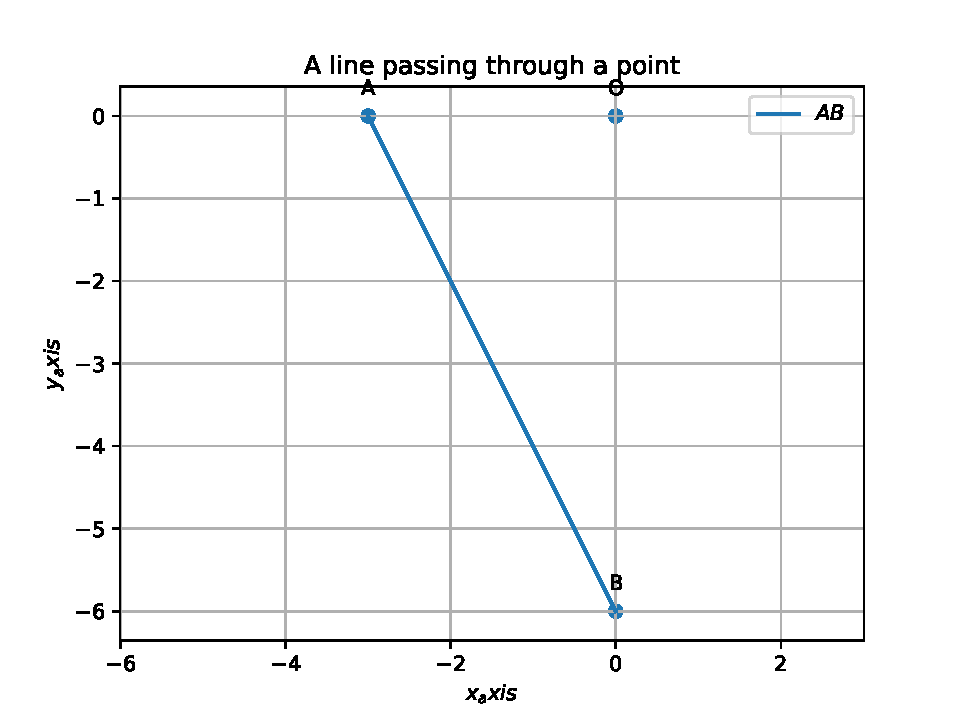
\includegraphics[width=\columnwidth]{line1.pdf}
%	  \caption{}
%	  \label{fig:line1.pdf}
%	  \end{figure} 	 		  


\item Show that the line through the points $(4,7,8),(2,3,4)$ is parallel to the line through the points $(-1,-2,1),(1,2,5)$.\\
\item  Find the equation of the line which passes through the point $(1,2,3)$ and is parallel to the vector $3\hat{i}+2\hat{j}-2\hat{k}$\\
\item  Find the equation of the line in vector and in cartesian form that passes through the point with position vector $2\hat{i}-\hat{j}+4\hat{k}$ and is in direction $\hat{i}+2\hat{j}-\hat{k}$.\\
\item Find the cartesian equation of the line which passes through the point $(-2,4,-5)$ and parallel to the line given by$ \frac{x+3}{3}=\frac{y-4}{5}=\frac{z+8}{6}$.\\
\item The cartesian equation of a line is $ \frac{x-5}{3}=\frac{y+4}{7}=\frac{z-6}{2}$. Write its vector form.\\
\item Find the vector and the cartesian equations of the lines that passes through the origin and $(5,-2,3)$.\\
    \solution
		\iffalse
\documentclass[A4,12pt,twocolumn]{IEEEtran}
%
\usepackage{setspace}
\usepackage{gensymb}
%\doublespacing
\singlespacing

%\usepackage{graphicx}
%\usepackage{amssymb}
%\usepackage{relsize}
\usepackage[cmex10]{amsmath}
%\usepackage{amsthm}
%\interdisplaylinepenalty=2500
%\savesymbol{iint}
%\usepackage{txfonts}
%\restoresymbol{TXF}{iint}
%\usepackage{wasysym}
\usepackage{amsthm}
%\usepackage{iithtlc}
\usepackage{mathrsfs}
\usepackage{txfonts}
\usepackage{stfloats}
\usepackage{bm}
\usepackage{cite}
\usepackage{cases}
\usepackage{subfig}
%\usepackage{xtab}
\usepackage{longtable}
\usepackage{multirow}
%\usepackage{algorithm}
%\usepackage{algpseudocode}
\usepackage{enumitem}
\usepackage{mathtools}
\usepackage{steinmetz}
\usepackage{tikz}
\usepackage{circuitikz}
\usepackage{verbatim}
\usepackage{tfrupee}
\usepackage[breaklinks=true]{hyperref}
%\usepackage{stmaryrd}
\usepackage{tkz-euclide} % loads  TikZ and tkz-base
%\usetkzobj{all}
\usetikzlibrary{calc,math}
\usepackage{listings}
    \usepackage{color}                                            %%
    \usepackage{array}                                            %%
    \usepackage{longtable}                                        %%
    \usepackage{calc}                                             %%
    \usepackage{multirow}                                         %%
    \usepackage{hhline}                                           %%
    \usepackage{ifthen}                                           %%
  %optionally (for landscape tables embedded in another document): %%
    \usepackage{lscape}     
\usepackage{multicol}
\usepackage{chngcntr}
%\usepackage{enumerate}

%\usepackage{wasysym}
%\newcounter{MYtempeqncnt}
\DeclareMathOperator*{\Res}{Res}
%\renewcommand{\baselinestretch}{2}
\renewcommand\thesection{\arabic{section}}
\renewcommand\thesubsection{\thesection.\arabic{subsection}}
\renewcommand\thesubsubsection{\thesubsection.\arabic{subsubsection}}

\renewcommand\thesectiondis{\arabic{section}}
\renewcommand\thesubsectiondis{\thesectiondis.\arabic{subsection}}
\renewcommand\thesubsubsectiondis{\thesubsectiondis.\arabic{subsubsection}}

% correct bad hyphenation here
\hyphenation{op-tical net-works semi-conduc-tor}
\def\inputGnumericTable{}                                 %%

\lstset{
%language=C,
frame=single, 
breaklines=true,
columns=fullflexible
}
%\lstset{
%language=tex,
%frame=single, 
%breaklines=true
%}

\begin{document}
%


\newtheorem{theorem}{Theorem}[section]
\newtheorem{problem}{Problem}
\newtheorem{proposition}{Proposition}[section]
\newtheorem{lemma}{Lemma}[section]
\newtheorem{corollary}[theorem]{Corollary}
\newtheorem{example}{Example}[section]
\newtheorem{definition}[problem]{Definition}
%\newtheorem{thm}{Theorem}[section] 
%\newtheorem{defn}[thm]{Definition}
%\newtheorem{algorithm}{Algorithm}[section]
%\newtheorem{cor}{Corollary}
\newcommand{\BEQA}{\begin{eqnarray}}
\newcommand{\EEQA}{\end{eqnarray}}
\newcommand{\define}{\stackrel{\triangle}{=}}

\bibliographystyle{IEEEtran}
%\bibliographystyle{ieeetr}


\providecommand{\mbf}{\mathbf}
\providecommand{\pr}[1]{\ensuremath{\Pr\left(#1\right)}}
\providecommand{\qfunc}[1]{\ensuremath{Q\left(#1\right)}}
\providecommand{\sbrak}[1]{\ensuremath{{}\left[#1\right]}}
\providecommand{\lsbrak}[1]{\ensuremath{{}\left[#1\right.}}
\providecommand{\rsbrak}[1]{\ensuremath{{}\left.#1\right]}}
\providecommand{\brak}[1]{\ensuremath{\left(#1\right)}}
\providecommand{\lbrak}[1]{\ensuremath{\left(#1\right.}}
\providecommand{\rbrak}[1]{\ensuremath{\left.#1\right)}}
\providecommand{\cbrak}[1]{\ensuremath{\left\{#1\right\}}}
\providecommand{\lcbrak}[1]{\ensuremath{\left\{#1\right.}}
\providecommand{\rcbrak}[1]{\ensuremath{\left.#1\right\}}}
\theoremstyle{remark}
\newtheorem{rem}{Remark}
\newcommand{\sgn}{\mathop{\mathrm{sgn}}}
\providecommand{\abs}[1]{\left\vert#1\right\vert}
\providecommand{\res}[1]{\Res\displaylimits_{#1}} 
\providecommand{\norm}[1]{\left\lVert#1\right\rVert}
%\providecommand{\norm}[1]{\lVert#1\rVert}
\providecommand{\mtx}[1]{\mathbf{#1}}
\providecommand{\mean}[1]{E\left[ #1 \right]}
\providecommand{\fourier}{\overset{\mathcal{F}}{ \rightleftharpoons}}
%\providecommand{\hilbert}{\overset{\mathcal{H}}{ \rightleftharpoons}}
\providecommand{\system}{\overset{\mathcal{H}}{ \longleftrightarrow}}
	%\newcommand{\solution}[2]{\textbf{Solution:}{#1}}
\newcommand{\solution}{\noindent \textbf{Solution: }}
\newcommand{\cosec}{\,\text{cosec}\,}
\providecommand{\dec}[2]{\ensuremath{\overset{#1}{\underset{#2}{\gtrless}}}}
\newcommand{\myvec}[1]{\ensuremath{\begin{pmatrix}#1\end{pmatrix}}}
\newcommand{\mydet}[1]{\ensuremath{\begin{vmatrix}#1\end{vmatrix}}}
%\numberwithin{equation}{section}
\numberwithin{equation}{subsection}
%\numberwithin{problem}{section}
%\numberwithin{definition}{section}
\makeatletter
\@addtoreset{figure}{problem}
\makeatother

\let\StandardTheFigure\thefigure
\let\vec\mathbf
%\renewcommand{\thefigure}{\theproblem.\arabic{figure}}
\renewcommand{\thefigure}{\theproblem}
%\setlist[enumerate,1]{before=\renewcommand\theequation{\theenumi.\arabic{equation}}
%\counterwithin{equation}{enumi}


%\renewcommand{\theequation}{\arabic{subsection}.\arabic{equation}}

\def\putbox#1#2#3{\makebox[0in][l]{\makebox[#1][l]{}\raisebox{\baselineskip}[0in][0in]{\raisebox{#2}[0in][0in]{#3}}}}
     \def\rightbox#1{\makebox[0in][r]{#1}}
     \def\centbox#1{\makebox[0in]{#1}}
     \def\topbox#1{\raisebox{-\baselineskip}[0in][0in]{#1}}
     \def\midbox#1{\raisebox{-0.5\baselineskip}[0in][0in]{#1}}

\vspace{3cm}


\title{QUIZ 4}
\author{Shristy Sharma (EE22BNITS11001)}





% make the title area
\maketitle

\newpage

%\tableofcontents

\bigskip

\renewcommand{\thefigure}{\theenumi}
\renewcommand{\thetable}{\theenumi}
%\renewcommand{\theequation}{\theenumi}


%Download all python codes 
%
%\begin{lstlisting}
%svn co https://github.com/JayatiD93/trunk/My_solution_design/codes
%\end{lstlisting}

%Download all and latex-tikz codes from 
%
%\begin{lstlisting}
%svn co https://github.com/gadepall/school/trunk/ncert/geometry/figs
%\end{lstlisting}
%


\section{PROBLEM 1}
1.  Find the vector and the cartesian equations of the lines that passes through the
origin and \myvec{5\\– 2\\3}.
\\SOLUTION:\\
\fi
Let
\begin{align}
\vec{A}=\myvec{0\\0\\0},\,
\vec{B}=\myvec{5\\-2\\3}
\end{align}
Then the desired line is given by 
\begin{align}
\vec{x}=\vec{A}+\lambda\vec{B}
=\lambda\myvec{5\\-2\\3}
\end{align}




\item Find the vector and the cartesian equations of the line that passes through the points $(3,-2,-5),(3,-2,6)$.\\
    \solution
		\iffalse
\documentclass[journal,12pt,twocolumn]{IEEEtran}
\usepackage{setspace}
\usepackage{gensymb}
\usepackage{xcolor}
\usepackage{caption}
\singlespacing
\usepackage{siunitx}
\usepackage[cmex10]{amsmath}
\usepackage{mathtools}
\usepackage{hyperref}
\usepackage{amsthm}
\usepackage{mathrsfs}
\usepackage{txfonts}
\usepackage{stfloats}
\usepackage{cite}
\usepackage{cases}
\usepackage{subfig}
\usepackage{longtable}
\usepackage{multirow}
\usepackage{enumitem}
\usepackage{bm}
\usepackage{mathtools}
\usepackage{listings}
\usepackage{tikz}
\usetikzlibrary{shapes,arrows,positioning}
\usepackage{circuitikz}
\renewcommand{\vec}[1]{\boldsymbol{\mathbf{#1}}}
\DeclareMathOperator*{\Res}{Res}
\renewcommand\thesection{\arabic{section}}
\renewcommand\thesubsection{\thesection.\arabic{subsection}}
\renewcommand\thesubsubsection{\thesubsection.\arabic{subsubsection}}

\renewcommand\thesectiondis{\arabic{section}}
\renewcommand\thesubsectiondis{\thesectiondis.\arabic{subsection}}
\renewcommand\thesubsubsectiondis{\thesubsectiondis.\arabic{subsubsection}}
\hyphenation{op-tical net-works semi-conduc-tor}

\lstset{
language=Python,
frame=single, 
breaklines=true,
columns=fullflexible
}
\begin{document}
\theoremstyle{definition}
\newtheorem{theorem}{Theorem}[section]
\newtheorem{problem}{Problem}
\newtheorem{proposition}{Proposition}[section]
\newtheorem{lemma}{Lemma}[section]
\newtheorem{corollary}[theorem]{Corollary}
\newtheorem{example}{Example}[section]
\newtheorem{definition}{Definition}[section]
\newcommand{\BEQA}{\begin{eqnarray}}
        \newcommand{\EEQA}{\end{eqnarray}}
\newcommand{\define}{\stackrel{\triangle}{=}}
\newcommand{\myvec}[1]{\ensuremath{\begin{pmatrix}#1\end{pmatrix}}}
\newcommand{\mydet}[1]{\ensuremath{\begin{vmatrix}#1\end{vmatrix}}}
\bibliographystyle{IEEEtran}
\providecommand{\nCr}[2]{\,^{#1}C_{#2}} % nCr
\providecommand{\nPr}[2]{\,^{#1}P_{#2}} % nPr
\providecommand{\mbf}{\mathbf}
\providecommand{\pr}[1]{\ensuremath{\Pr\left(#1\right)}}
\providecommand{\qfunc}[1]{\ensuremath{Q\left(#1\right)}}
\providecommand{\sbrak}[1]{\ensuremath{{}\left[#1\right]}}
\providecommand{\lsbrak}[1]{\ensuremath{{}\left[#1\right.}}
\providecommand{\rsbrak}[1]{\ensuremath{{}\left.#1\right]}}
\providecommand{\brak}[1]{\ensuremath{\left(#1\right)}}
\providecommand{\lbrak}[1]{\ensuremath{\left(#1\right.}}
\providecommand{\rbrak}[1]{\ensuremath{\left.#1\right)}}
\providecommand{\cbrak}[1]{\ensuremath{\left\{#1\right\}}}
\providecommand{\lcbrak}[1]{\ensuremath{\left\{#1\right.}}
\providecommand{\rcbrak}[1]{\ensuremath{\left.#1\right\}}}
\theoremstyle{remark}
\newtheorem{rem}{Remark}
\newcommand{\sgn}{\mathop{\mathrm{sgn}}}
\newcommand{\rect}{\mathop{\mathrm{rect}}}
\newcommand{\sinc}{\mathop{\mathrm{sinc}}}
\providecommand{\abs}[1]{\left\vert#1\right\vert}
\providecommand{\res}[1]{\Res\displaylimits_{#1}}
\providecommand{\norm}[1]{\lVert#1\rVert}
\providecommand{\mtx}[1]{\mathbf{#1}}
\providecommand{\mean}[1]{E\left[ #1 \right]}
\providecommand{\fourier}{\overset{\mathcal{F}}{ \rightleftharpoons}}
\providecommand{\ztrans}{\overset{\mathcal{Z}}{ \rightleftharpoons}}
\providecommand{\system}[1]{\overset{\mathcal{#1}}{ \longleftrightarrow}}
\newcommand{\solution}{\noindent \textbf{Solution: }}
\providecommand{\dec}[2]{\ensuremath{\overset{#1}{\underset{#2}{\gtrless}}}}
\let\StandardTheFigure\thefigure
\def\putbox#1#2#3{\makebox[0in][l]{\makebox[#1][l]{}\raisebox{\baselineskip}[0in][0in]{\raisebox{#2}[0in][0in]{#3}}}}
\def\rightbox#1{\makebox[0in][r]{#1}}
\def\centbox#1{\makebox[0in]{#1}}
\def\topbox#1{\raisebox{-\baselineskip}[0in][0in]{#1}}
\def\midbox#1{\raisebox{-0.5\baselineskip}[0in][0in]{#1}}

\vspace{3cm}
\title{12.11.2.9}
\author{Lokesh Surana}
\maketitle
\section*{Class 12, Chapter 11, Exercise 2.9}

Q.9. Find the vector equation of the line that passes through the points $\myvec{3\\-2\\-5}, \myvec{3\\-2\\6}$.
\solution 
\fi
The given points are
\begin{align}
    \vec{a} = \myvec{3\\-2\\-5},\, 
    \vec{b} = \myvec{3\\-2\\6}
\end{align}
The equation of line through $\vec{a} \text{ and } \vec{b}$ is given by,
\begin{align}
    \vec{r} &= \vec{a} + \lambda(\vec{b} - \vec{a}) 
 =  \myvec{3\\-2\\-5} + \lambda\myvec{3\\-2\\6} -\lambda\myvec{3\\-2\\-5} \\
 &= \myvec{3\\-2\\-5} + \lambda\myvec{0\\0\\11}
\end{align}
See Fig. 
    \ref{fig:chapters/12/11/2/9line}.
\begin{figure}[!htb]
    \centering
    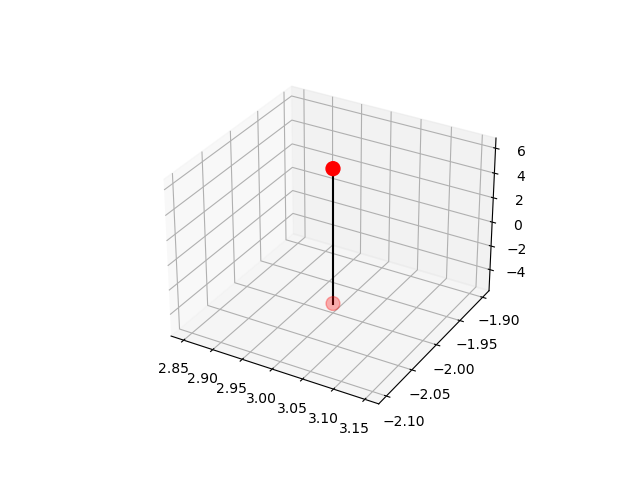
\includegraphics[width=\columnwidth]{chapters/12/11/2/9/figs/line.png}
    \caption{Line passing through (3, -2, -5) and (3, -2, 6)}
    \label{fig:chapters/12/11/2/9line}
\end{figure}


\item  Find the angle between the following pairs of lines:
\begin{enumerate}
\item  $\overrightarrow{r}=2\hat{i}-5\hat{j}+\hat{k}+\lambda(3\hat{i}+2\hat{j}+6\hat{k})$ and\\ $\overrightarrow{r}=7\hat{i}-6\hat{k}+\mu(\hat{i}+2\hat{j}+2\hat{k})$
\item   $\overrightarrow{r}=3\hat{i}+\hat{j}-2\hat{k}+\lambda(\hat{i}-\hat{j}-2\hat{k})$ and\\ $\overrightarrow{r}=2\hat{i}-\hat{j}-56\hat{k}+\mu(3\hat{i}-5\hat{j}-4\hat{k})$ 
\end{enumerate}
\item Find the angle between the following pairs of lines:
\begin{enumerate}
\item $ \frac{x-2}{2}=\frac{y-1}{5}=\frac{z+3}{-3}$ and $ \frac{x+2}{-1}=\frac{y-4}{8}=\frac{z-5}{4}$.
\item $ \frac{x}{2}=\frac{y}{2}=\frac{z}{1}$ and $ \frac{x-5}{4}=\frac{y-2}{1}=\frac{z-3}{8}$.
\end{enumerate}
\item Find the values of p so that the lines $ \frac{1-x}{3}=\frac{7y-14}{2p}=\frac{z-3}{2}$ and $ \frac{7-7x}{3p}=\frac{y-5}{1}=\frac{6-z}{5}$ are at right angles.
\item Show that the lines $ \frac{x-5}{7}=\frac{y+2}{-5}=\frac{z}{1}$ and $ \frac{x}{1}=\frac{y}{2}=\frac{z}{3}$ are perpendicular to each other.
\item Find the shortest distance between the lines\\  $\overrightarrow{r}=(\hat{i}+2\hat{j}+\hat{k})+\lambda(\hat{i}-\hat{j}+\hat{k})$ and \\$\overrightarrow{r}=2\hat{i}-\hat{j}-\hat{k}+\mu(2\hat{i}+\hat{j}+2\hat{k})$
\item Find the shortest distance between the lines\\
$ \frac{x+1}{7}=\frac{y+1}{-6}=\frac{z+1}{1}$ and $ \frac{x-3}{1}=\frac{y-5}{-2}=\frac{z-7}{1}$ 
    \solution
		\iffalse
\documentclass[journal,12pt,twocolumn]{IEEEtran}
\usepackage{romannum}
\usepackage{float}
\usepackage{setspace}
\usepackage{gensymb}
\singlespacing
\usepackage[cmex10]{amsmath}
\usepackage{amsthm}
\usepackage{mathrsfs}
\usepackage{txfonts}
\usepackage{stfloats}
\usepackage{bm}
\usepackage{cite}
\usepackage{cases}
\usepackage{subfig}
\usepackage{longtable}
\usepackage{multirow}
\usepackage{enumitem}
\usepackage{mathtools}
\usepackage{steinmetz}
\usepackage{tikz}
\usepackage{circuitikz}
\usepackage{verbatim}
\usepackage{tfrupee}
\usepackage[breaklinks=true]{hyperref}
\usepackage{tkz-euclide}
\usetikzlibrary{calc,math}
\usepackage{listings}
    \usepackage{color}                                            %%
    \usepackage{array}                                            %%
    \usepackage{longtable}                                        %%
    \usepackage{calc}                                             %%
    \usepackage{multirow}                                         %%
    \usepackage{hhline}                                           %%
    \usepackage{ifthen}                                           %%
  %optionally (for landscape tables embedded in another document): %%
    \usepackage{lscape}     
\usepackage{multicol}
\usepackage{chngcntr}
\DeclareMathOperator*{\Res}{Res}
\renewcommand\thesection{\arabic{section}}
\renewcommand\thesubsection{\thesection.\arabic{subsection}}
\renewcommand\thesubsubsection{\thesubsection.\arabic{subsubsection}}

\renewcommand\thesectiondis{\arabic{section}}
\renewcommand\thesubsectiondis{\thesectiondis.\arabic{subsection}}
\renewcommand\thesubsubsectiondis{\thesubsectiondis.\arabic{subsubsection}}

% correct bad hyphenation here
\hyphenation{op-tical net-works semi-conduc-tor}
\def\inputGnumericTable{}                                 %%

\lstset{
frame=single, 
breaklines=true,
columns=fullflexible
}

\begin{document}


\newtheorem{theorem}{Theorem}[section]
\newtheorem{problem}{Problem}
\newtheorem{proposition}{Proposition}[section]
\newtheorem{lemma}{Lemma}[section]
\newtheorem{corollary}[theorem]{Corollary}
\newtheorem{example}{Example}[section]
\newtheorem{definition}[problem]{Definition}
\newcommand{\BEQA}{\begin{eqnarray}}
\newcommand{\EEQA}{\end{eqnarray}}
\newcommand{\define}{\stackrel{\triangle}{=}}

\bibliographystyle{IEEEtran}
\providecommand{\mbf}{\mathbf}
\providecommand{\pr}[1]{\ensuremath{\Pr\left(#1\right)}}
\providecommand{\qfunc}[1]{\ensuremath{Q\left(#1\right)}}
\providecommand{\sbrak}[1]{\ensuremath{{}\left[#1\right]}}
\providecommand{\lsbrak}[1]{\ensuremath{{}\left[#1\right.}}
\providecommand{\rsbrak}[1]{\ensuremath{{}\left.#1\right]}}
\providecommand{\brak}[1]{\ensuremath{\left(#1\right)}}
\providecommand{\lbrak}[1]{\ensuremath{\left(#1\right.}}
\providecommand{\rbrak}[1]{\ensuremath{\left.#1\right)}}
\providecommand{\cbrak}[1]{\ensuremath{\left\{#1\right\}}}
\providecommand{\lcbrak}[1]{\ensuremath{\left\{#1\right.}}
\providecommand{\rcbrak}[1]{\ensuremath{\left.#1\right\}}}
\theoremstyle{remark}
\newtheorem{rem}{Remark}
\newcommand{\sgn}{\mathop{\mathrm{sgn}}}
\providecommand{\abs}[1]{\left\vert#1\right\vert}
\providecommand{\res}[1]{\Res\displaylimits_{#1}} 
\providecommand{\norm}[1]{\left\lVert#1\right\rVert}
\providecommand{\mtx}[1]{\mathbf{#1}}
\providecommand{\mean}[1]{E\left[ #1 \right]}
\providecommand{\fourier}{\overset{\mathcal{F}}{ \rightleftharpoons}}
\providecommand{\system}{\overset{\mathcal{H}}{ \longleftrightarrow}}
\newcommand{\solution}{\noindent \textbf{Solution: }}
\newcommand{\cosec}{\,\text{cosec}\,}
\providecommand{\dec}[2]{\ensuremath{\overset{#1}{\underset{#2}{\gtrless}}}}
\newcommand{\myvec}[1]{\ensuremath{\begin{pmatrix}#1\end{pmatrix}}}
\newcommand{\mydet}[1]{\ensuremath{\begin{vmatrix}#1\end{vmatrix}}}
\numberwithin{equation}{subsection}
\makeatletter
\@addtoreset{figure}{problem}
\makeatother

\let\StandardTheFigure\thefigure
\let\vec\mathbf
\renewcommand{\thefigure}{\theproblem}



\def\putbox#1#2#3{\makebox[0in][l]{\makebox[#1][l]{}\raisebox{\baselineskip}[0in][0in]{\raisebox{#2}[0in][0in]{#3}}}}
     \def\rightbox#1{\makebox[0in][r]{#1}}
     \def\centbox#1{\makebox[0in]{#1}}
     \def\topbox#1{\raisebox{-\baselineskip}[0in][0in]{#1}}
     \def\midbox#1{\raisebox{-0.5\baselineskip}[0in][0in]{#1}}

\vspace{3cm}


\title{Question: 12.11.2.15}
\author{Nikam Pratik Balasaheb (EE21BTECH11037)}





% make the title area
\maketitle

\newpage

%\tableofcontents

\bigskip

\renewcommand{\thefigure}{\theenumi}
\renewcommand{\thetable}{\theenumi}

\section{Problem}
Find the shortest distance between the lines $\frac{x+1}{7} = \frac{y+1}{-6}=\frac{z+1}{1}$ and $\frac{x-3}{1} = \frac{y-5}{-2}=\frac{z-7}{1}$

\section{Solution}
\fi
 The given lines  can be written as
\begin{align}
\vec{x} &= \myvec{-1\\-1\\-1} + \lambda_1\myvec{7\\-6\\1}\\
\vec{x} &= \myvec{3\\5\\7} + \lambda_2\myvec{1\\-2\\1} \\
\vec{x_1} = \myvec{-1\\-1\\-1},\, \vec{x_2} &= \myvec{3\\5\\7}, \,\vec{m_1} = \myvec{7\\-6\\1}, \, \vec{m_2} = \myvec{1\\-2\\1}
\end{align}
%
We first check whether the given lines are skew. The lines 
\begin{align}
\vec{x} = \vec{x_1} + \lambda_1\vec{m_1},\, \vec{x} = \vec{x_2} + \lambda_2\vec{m_2} 
\label{eq:chapters/12/11/2/15/1}
\end{align}
intersect if
\begin{align}
\vec{M}{\lambda} &= \vec{x_2} - \vec{x_1}\\
\vec{M} &\triangleq \myvec{\vec{m_1} & \vec{m_2}} \\
\bm{\lambda} &\triangleq \myvec{\lambda_1\\-\lambda_2}\\
\end{align}
Here we have,
\begin{align}
\vec{M} = \myvec{7&1\\-6&-2\\1&1}\,
\vec{x_2} - \vec{x_1} = \myvec{4\\6\\8}
\end{align}
We check whether the equation \eqref{eq:chapters/12/11/2/15/2} has a solution
\begin{align}
\myvec{7&1\\-6&-2\\1&1}\bm{\lambda} = \myvec{4\\6\\8}
\label{eq:chapters/12/11/2/15/2}
\end{align}
the augmented matrix is given by,
\begin{align}
\myvec{7&1&\vrule&4\\-6&-2&\vrule&6\\1&1&\vrule&8}
\xleftrightarrow[R_3 \leftarrow R_3 - \frac{1}{7}R_1]{R_2 \leftarrow R_2 + \frac{6}{7}R_1}\\
\myvec{7&1&\vrule&4\\&&\vrule\\0&-\frac{8}{7}&\vrule&\frac{66}{7}\\&&\vrule\\0&\frac{6}{7}&\vrule&-\frac{52}{7}}
\xleftrightarrow{R_3 \leftarrow R_3 + \frac{3}{4}R_2}\\
\myvec{2&3&\vrule&1\\&&\vrule\\0&-\frac{7}{2}&\vrule&\frac{1}{2}\\&&\vrule\\0&0&\vrule&-\frac{5}{14}}
\end{align}
The rank of the matrix is 3. So the given lines are skew.
The closest points on two skew lines defined by \eqref{eq:chapters/12/11/2/15/1} are given by 
\begin{align}
\vec{M}^\top \vec{M}\bm{\lambda} &= \vec{M}^\top\brak{\vec{x_2}-\vec{x_1}}\\
\implies \myvec{7&-6&1\\1&-2&1} \myvec{7&1\\-6&-2\\1&1}\bm{\lambda} &= \myvec{7&-6&1\\1&-2&1} \myvec{4\\6\\8}\\
\implies \myvec{86&20\\20&6}\bm{\lambda} &= \myvec{0\\0}
\label{eq:chapters/12/11/2/15/3}
\end{align}
The augmented matrix of the above equation \eqref{eq:chapters/12/11/2/15/3} is given by,
\begin{align}
\myvec{86&20&\vrule&0\\20&6&\vrule&0}
\xleftrightarrow{R_2 \leftarrow R_2 - \frac{10}{43}R_1}
\myvec{86&20&\vrule&0 \\&&\vrule\\ 0&\frac{58}{43}&\vrule&0}
\xleftrightarrow[R_2 \leftarrow \frac{43}{58}R_2]{R_1 \leftarrow \frac{1}{86} \brak{R_1 - \frac{430}{29}R_2}}\\
\myvec{1&0&\vrule&0 \\&&\vrule\\ 0&1&\vrule&0}
\end{align}
yielding
\begin{align}
\myvec{\lambda_1\\-\lambda_2} &= \myvec{0\\0}
\end{align}
The closest points $\vec{A}$ on line $l_1$ and $\vec{B}$ on line $l_2$ are given by,
\begin{align}
\vec{A} &= \vec{x_1} + \lambda_1\vec{m_1}
= \myvec{-1\\-1\\-1}\\
\vec{B} &= \vec{x_2} + \lambda_2\vec{m_2}
= \myvec{3\\5\\7}
\end{align}
The minimum distance between the lines is given by
\begin{align}
\norm{\vec{B}-\vec{A}} &= \norm{\myvec{4\\6\\8}}
= 2\sqrt{29}
\end{align}
%
\begin{figure}[!ht]
\centering
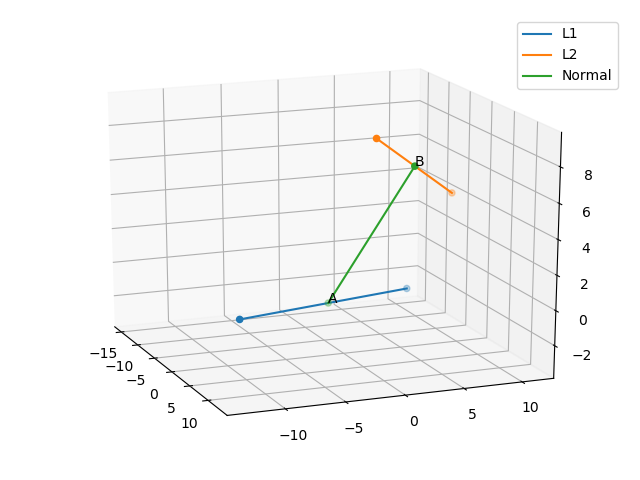
\includegraphics[width=\columnwidth]{chapters/12/11/2/15/figs/Figure_1.png}
\caption{}
\label{fig:chapters/12/11/2/15/}
\end{figure}


    \item Find the shortest distance between the lines whose vector equations are
    \begin{align}
        \vec{x} = \myvec{1\\2\\3} + \lambda_1\myvec{1\\-3\\2}
        \label{eq:chapters/12/11/2/16/L1}
    \end{align}
    and
    \begin{align}
        \vec{x} = \myvec{4\\5\\6} + \lambda_2\myvec{2\\3\\1}
        \label{eq:chapters/12/11/2/16/L2}
    \end{align}
    \solution
		\iffalse
\documentclass[journal,12pt,twocolumn]{IEEEtran}
\usepackage{setspace}
\usepackage{gensymb}
\usepackage{xcolor}
\usepackage{caption}
\singlespacing
\usepackage{siunitx}
\usepackage[cmex10]{amsmath}
\usepackage{mathtools}
\usepackage{hyperref}
\usepackage{amsthm}
\usepackage{mathrsfs}
\usepackage{txfonts}
\usepackage{stfloats}
\usepackage{cite}
\usepackage{cases}
\usepackage{subfig}
\usepackage{longtable}
\usepackage{multirow}
\usepackage{enumitem}
\usepackage{bm}
\usepackage{mathtools}
\usepackage{listings}
\usepackage{tikz}
\usetikzlibrary{shapes,arrows,positioning}
\usepackage{circuitikz}
\renewcommand{\vec}[1]{\boldsymbol{\mathbf{#1}}}
\DeclareMathOperator*{\Res}{Res}
\renewcommand\thesection{\arabic{section}}
\renewcommand\thesubsection{\thesection.\arabic{subsection}}
\renewcommand\thesubsubsection{\thesubsection.\arabic{subsubsection}}

\renewcommand\thesectiondis{\arabic{section}}
\renewcommand\thesubsectiondis{\thesectiondis.\arabic{subsection}}
\renewcommand\thesubsubsectiondis{\thesubsectiondis.\arabic{subsubsection}}
\hyphenation{op-tical net-works semi-conduc-tor}

\lstset{
language=Python,
frame=single, 
breaklines=true,
columns=fullflexible
}
\begin{document}
\theoremstyle{definition}
\newtheorem{theorem}{Theorem}[section]
\newtheorem{problem}{Problem}
\newtheorem{proposition}{Proposition}[section]
\newtheorem{lemma}{Lemma}[section]
\newtheorem{corollary}[theorem]{Corollary}
\newtheorem{example}{Example}[section]
\newtheorem{definition}{Definition}[section]
\newcommand{\BEQA}{\begin{eqnarray}}
\newcommand{\EEQA}{\end{eqnarray}}
\newcommand{\define}{\stackrel{\triangle}{=}}
\newcommand{\myvec}[1]{\ensuremath{\begin{pmatrix}#1\end{pmatrix}}}
\newcommand{\mydet}[1]{\ensuremath{\begin{vmatrix}#1\end{vmatrix}}}
\bibliographystyle{IEEEtran}
\providecommand{\nCr}[2]{\,^{#1}C_{#2}} % nCr
\providecommand{\nPr}[2]{\,^{#1}P_{#2}} % nPr
\providecommand{\mbf}{\mathbf}
\providecommand{\pr}[1]{\ensuremath{\Pr\left(#1\right)}}
\providecommand{\qfunc}[1]{\ensuremath{Q\left(#1\right)}}
\providecommand{\sbrak}[1]{\ensuremath{{}\left[#1\right]}}
\providecommand{\lsbrak}[1]{\ensuremath{{}\left[#1\right.}}
\providecommand{\rsbrak}[1]{\ensuremath{{}\left.#1\right]}}
\providecommand{\brak}[1]{\ensuremath{\left(#1\right)}}
\providecommand{\lbrak}[1]{\ensuremath{\left(#1\right.}}
\providecommand{\rbrak}[1]{\ensuremath{\left.#1\right)}}
\providecommand{\cbrak}[1]{\ensuremath{\left\{#1\right\}}}
\providecommand{\lcbrak}[1]{\ensuremath{\left\{#1\right.}}
\providecommand{\rcbrak}[1]{\ensuremath{\left.#1\right\}}}
\theoremstyle{remark}
\newtheorem{rem}{Remark}
\newcommand{\sgn}{\mathop{\mathrm{sgn}}}
\newcommand{\rect}{\mathop{\mathrm{rect}}}
\newcommand{\sinc}{\mathop{\mathrm{sinc}}}
\providecommand{\abs}[1]{\left\vert#1\right\vert}
\providecommand{\res}[1]{\Res\displaylimits_{#1}} 
\providecommand{\norm}[1]{\lVert#1\rVert}
\providecommand{\mtx}[1]{\mathbf{#1}}
\providecommand{\mean}[1]{E\left[ #1 \right]}
\providecommand{\fourier}{\overset{\mathcal{F}}{ \rightleftharpoons}}
\providecommand{\ztrans}{\overset{\mathcal{Z}}{ \rightleftharpoons}}
\providecommand{\system}[1]{\overset{\mathcal{#1}}{ \longleftrightarrow}}
\newcommand{\solution}{\noindent \textbf{Solution: }}
\providecommand{\dec}[2]{\ensuremath{\overset{#1}{\underset{#2}{\gtrless}}}}
\let\StandardTheFigure\thefigure
\def\putbox#1#2#3{\makebox[0in][l]{\makebox[#1][l]{}\raisebox{\baselineskip}[0in][0in]{\raisebox{#2}[0in][0in]{#3}}}}
     \def\rightbox#1{\makebox[0in][r]{#1}}
     \def\centbox#1{\makebox[0in]{#1}}
     \def\topbox#1{\raisebox{-\baselineskip}[0in][0in]{#1}}
     \def\midbox#1{\raisebox{-0.5\baselineskip}[0in][0in]{#1}}

\vspace{3cm}
\title{Line Assignment}
\author{Gautam Singh}
\maketitle
\bigskip

\begin{abstract}
    This document contains the solution to Question 16 of Exercise 2 in Chapter
    11 of the class 12 NCERT textbook.
\end{abstract}
\fi
    In this case,
    \begin{align}
        \vec{x_1} = \myvec{1\\2\\3} \quad \vec{x_2} = \myvec{4\\5\\6}
        \quad \vec{m_1} = \myvec{1\\-3\\2} \quad \vec{m_2} = \myvec{2\\3\\1}
        \label{eq:chapters/12/11/2/16/vals}
    \end{align}
    To check whether \eqref{eq:chapters/12/11/2/16/intersect-cond} has a solution in $\vec{\lambda}$,
    we use the augmented matrix.
    \begin{align}
        \myvec{1&2&3\\-3&3&3\\2&1&3} &\xleftrightarrow[]{R_2\leftarrow R_2+3R_1} \myvec{1&2&3\\0&9&12\\2&1&3} \\
                &\xleftrightarrow[]{R_3\leftarrow R_3-2R_1} \myvec{1&2&3\\0&9&12\\0&-3&-3} \\
                &\xleftrightarrow[]{R_3\leftarrow 3R_3+R_2} \myvec{1&2&3\\0&9&12\\0&0&3}
                \label{eq:chapters/12/11/2/16/rank-aug}
    \end{align}
    Clearly, the rank of this matrix is 3, and therefore, the lines are skew.
%
    Substituting from \eqref{eq:chapters/12/11/2/16/vals} in \eqref{eq:chapters/12/11/2/16/lambda-eqn} and forming the 
    augmented matrix,
    \begin{align}
        \myvec{14&-5&0\\-5&14&18} &\xleftrightarrow[]{R_1\leftarrow R_1+R_2} \myvec{9&9&18\\-5&14&18} \\
                 &\xleftrightarrow[]{R_1\leftarrow\frac{R_1}{9}} \myvec{1&1&2\\-5&14&18} \\
                 &\xleftrightarrow[]{R_2\leftarrow R_2+5R_1} \myvec{1&1&2\\0&19&28} \\
                 &\xleftrightarrow[]{R_1\leftarrow19R_1-R_2} \myvec{19&0&10\\0&19&28} \\
                 &\xleftrightarrow[]{\substack{R_1\leftarrow\frac{R_1}{19}\\R_2\leftarrow\frac{R_2}{9}}}
                    \myvec{1&0&\frac{10}{19}\\0&1&\frac{28}{19}} \\
                    \implies \vec{\lambda} &= \frac{1}{19}\myvec{10\\28}
        \label{eq:chapters/12/11/2/16/lambda-sol}
    \end{align}
    Hence, using \eqref{eq:chapters/12/11/2/16/lambda-def} and substituing into \eqref{eq:chapters/12/11/2/16/a-def} and \eqref{eq:chapters/12/11/2/16/b-def},
    \begin{align}
        \vec{A} = \frac{1}{19}\myvec{29\\8\\77} \quad \vec{B} = \frac{1}{19}\myvec{20\\11\\86}
    \end{align}
    Thus, the required distance is
    \begin{align}
        \norm{\vec{B}-\vec{A}} = \frac{\sqrt{9^2 +3^2 +(-9)^2}}{19} = \frac{3}{\sqrt{19}}
    \end{align}
    The situation is depicted in Fig. \ref{fig:chapters/12/11/2/16/skew}.

    \begin{figure}[!ht]
        \centering
        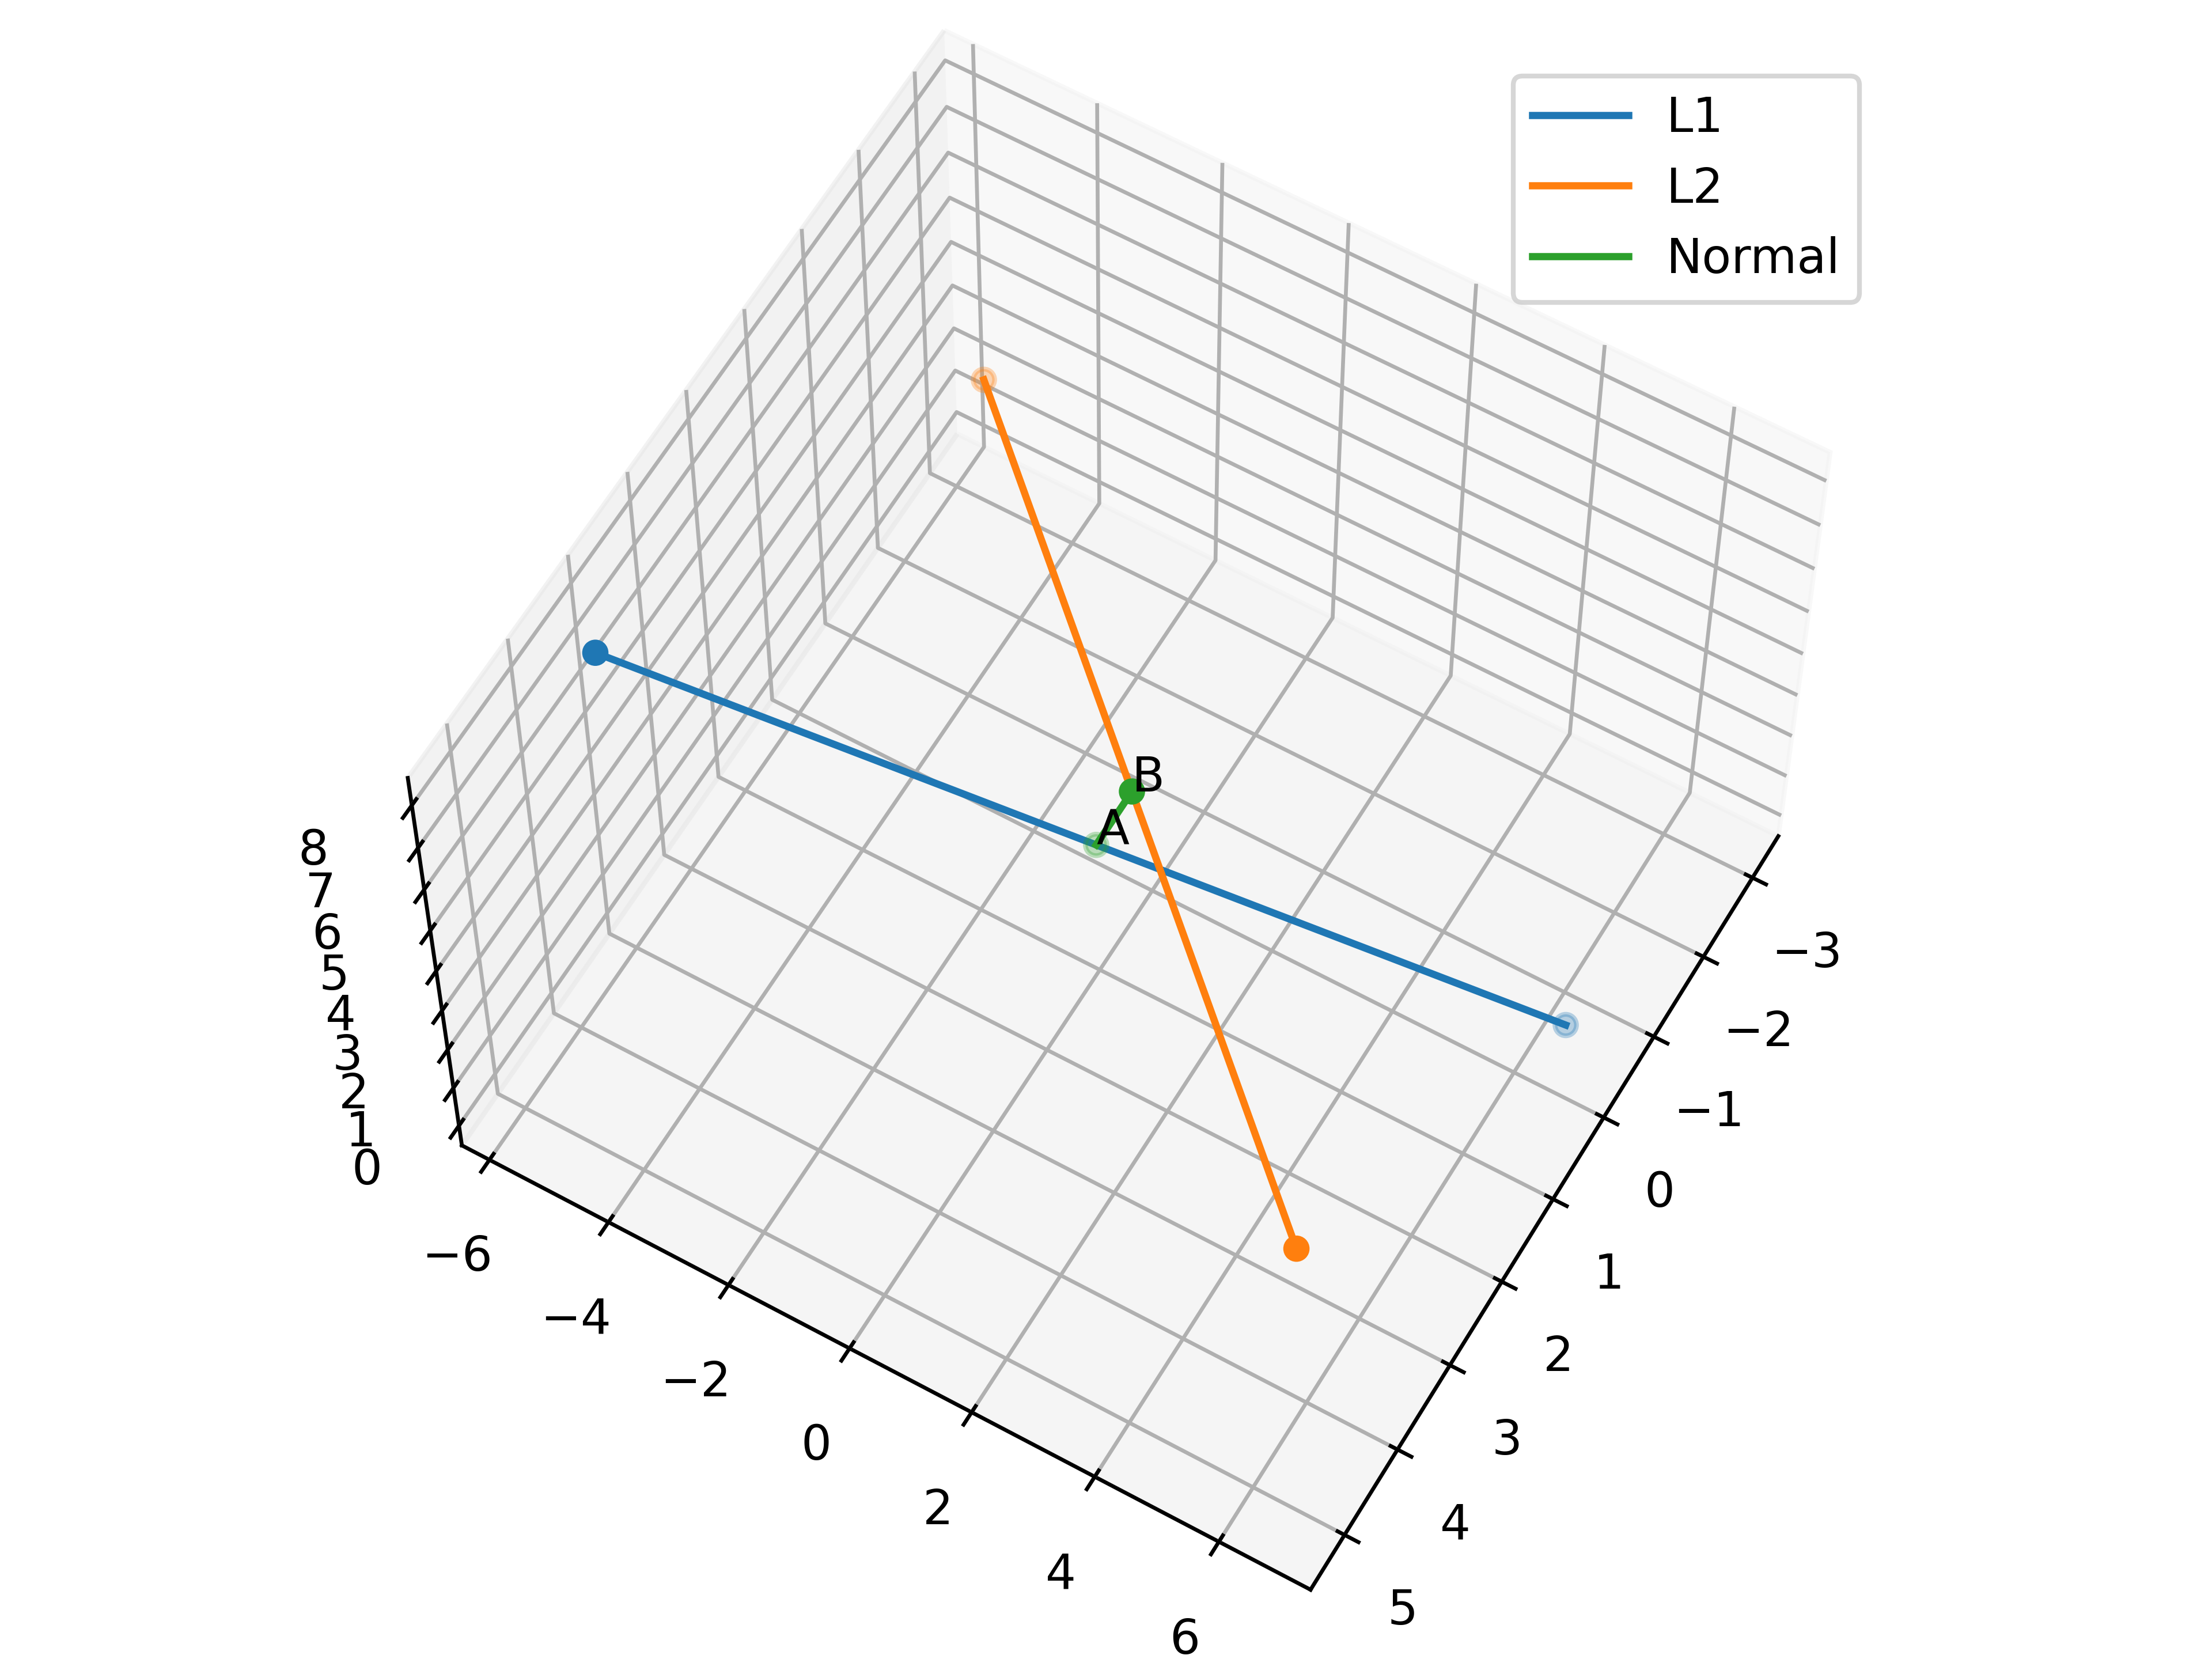
\includegraphics[width=\columnwidth]{chapters/12/11/2/16/figs/skew.png}
        \caption{$AB$ is the required shortest distance.}
        \label{fig:chapters/12/11/2/16/skew}
    \end{figure}

\item Find the shortest distance between the lines whose vector equations are \\
 $\overrightarrow{r}=(1-t)\hat{i}+(t-2)\hat{j}+(3-2t)\hat{k}$     and  \\$\overrightarrow{r}=(s+1)\hat{i}+(2s-1)\hat{j}-(2s+1)\hat{k}$
 \item 
\item Find the shortest distance between the lines $l_1$ and $l_2$ whose vector equations are ${\overrightarrow{r} = \hat{i}+\hat{j}+\lambda(2\hat{i}-\hat{j}+\hat{k})}$ and ${\overrightarrow{r} = 2\hat{i}+\hat{j}-\hat{k}+\mu(3\hat{i}-5\hat{j}+2\hat{k})}$.
    \solution
		\iffalse
\documentclass[journal,12pt,twocolumn]{IEEEtran}
\usepackage{romannum}
\usepackage{float}
\usepackage{setspace}
\usepackage{gensymb}
\singlespacing
\usepackage[cmex10]{amsmath}
\usepackage{amsthm}
\usepackage{mathrsfs}
\usepackage{txfonts}
\usepackage{stfloats}
\usepackage{bm}
\usepackage{cite}
\usepackage{cases}
\usepackage{subfig}
\usepackage{longtable}
\usepackage{multirow}
\usepackage{enumitem}
\usepackage{mathtools}
\usepackage{steinmetz}
\usepackage{tikz}
\usepackage{circuitikz}
\usepackage{verbatim}
\usepackage{tfrupee}
\usepackage[breaklinks=true]{hyperref}
\usepackage{tkz-euclide}
\usetikzlibrary{calc,math}
\usepackage{listings}
    \usepackage{color}                                            %%
    \usepackage{array}                                            %%
    \usepackage{longtable}                                        %%
    \usepackage{calc}                                             %%
    \usepackage{multirow}                                         %%
    \usepackage{hhline}                                           %%
    \usepackage{ifthen}                                           %%
  %optionally (for landscape tables embedded in another document): %%
    \usepackage{lscape}     
\usepackage{multicol}
\usepackage{chngcntr}
\DeclareMathOperator*{\Res}{Res}
\renewcommand\thesection{\arabic{section}}
\renewcommand\thesubsection{\thesection.\arabic{subsection}}
\renewcommand\thesubsubsection{\thesubsection.\arabic{subsubsection}}

\renewcommand\thesectiondis{\arabic{section}}
\renewcommand\thesubsectiondis{\thesectiondis.\arabic{subsection}}
\renewcommand\thesubsubsectiondis{\thesubsectiondis.\arabic{subsubsection}}

% correct bad hyphenation here
\hyphenation{op-tical net-works semi-conduc-tor}
\def\inputGnumericTable{}                                 %%

\lstset{
frame=single, 
breaklines=true,
columns=fullflexible
}

\begin{document}


\newtheorem{theorem}{Theorem}[section]
\newtheorem{problem}{Problem}
\newtheorem{proposition}{Proposition}[section]
\newtheorem{lemma}{Lemma}[section]
\newtheorem{corollary}[theorem]{Corollary}
\newtheorem{example}{Example}[section]
\newtheorem{definition}[problem]{Definition}
\newcommand{\BEQA}{\begin{eqnarray}}
\newcommand{\EEQA}{\end{eqnarray}}
\newcommand{\define}{\stackrel{\triangle}{=}}

\bibliographystyle{IEEEtran}
\providecommand{\mbf}{\mathbf}
\providecommand{\pr}[1]{\ensuremath{\Pr\left(#1\right)}}
\providecommand{\qfunc}[1]{\ensuremath{Q\left(#1\right)}}
\providecommand{\sbrak}[1]{\ensuremath{{}\left[#1\right]}}
\providecommand{\lsbrak}[1]{\ensuremath{{}\left[#1\right.}}
\providecommand{\rsbrak}[1]{\ensuremath{{}\left.#1\right]}}
\providecommand{\brak}[1]{\ensuremath{\left(#1\right)}}
\providecommand{\lbrak}[1]{\ensuremath{\left(#1\right.}}
\providecommand{\rbrak}[1]{\ensuremath{\left.#1\right)}}
\providecommand{\cbrak}[1]{\ensuremath{\left\{#1\right\}}}
\providecommand{\lcbrak}[1]{\ensuremath{\left\{#1\right.}}
\providecommand{\rcbrak}[1]{\ensuremath{\left.#1\right\}}}
\theoremstyle{remark}
\newtheorem{rem}{Remark}
\newcommand{\sgn}{\mathop{\mathrm{sgn}}}
\providecommand{\abs}[1]{\left\vert#1\right\vert}
\providecommand{\res}[1]{\Res\displaylimits_{#1}} 
\providecommand{\norm}[1]{\left\lVert#1\right\rVert}
\providecommand{\mtx}[1]{\mathbf{#1}}
\providecommand{\mean}[1]{E\left[ #1 \right]}
\providecommand{\fourier}{\overset{\mathcal{F}}{ \rightleftharpoons}}
\providecommand{\system}{\overset{\mathcal{H}}{ \longleftrightarrow}}
\newcommand{\solution}{\noindent \textbf{Solution: }}
\newcommand{\cosec}{\,\text{cosec}\,}
\providecommand{\dec}[2]{\ensuremath{\overset{#1}{\underset{#2}{\gtrless}}}}
\newcommand{\myvec}[1]{\ensuremath{\begin{pmatrix}#1\end{pmatrix}}}
\newcommand{\mydet}[1]{\ensuremath{\begin{vmatrix}#1\end{vmatrix}}}
\numberwithin{equation}{subsection}
\makeatletter
\@addtoreset{figure}{problem}
\makeatother

\let\StandardTheFigure\thefigure
\let\vec\mathbf
\renewcommand{\thefigure}{\theproblem}



\def\putbox#1#2#3{\makebox[0in][l]{\makebox[#1][l]{}\raisebox{\baselineskip}[0in][0in]{\raisebox{#2}[0in][0in]{#3}}}}
     \def\rightbox#1{\makebox[0in][r]{#1}}
     \def\centbox#1{\makebox[0in]{#1}}
     \def\topbox#1{\raisebox{-\baselineskip}[0in][0in]{#1}}
     \def\midbox#1{\raisebox{-0.5\baselineskip}[0in][0in]{#1}}

\vspace{3cm}


\title{Assignment 1}
\author{Jaswanth Chowdary Madala}





% make the title area
\maketitle

\newpage

%\tableofcontents

\bigskip

\renewcommand{\thefigure}{\theenumi}
\renewcommand{\thetable}{\theenumi}

\begin{enumerate}

\textbf{Solution:}
\fi
		The givne lines can be written  in vector form  as
\begin{align}
	\vec{x} &= \myvec{1\\1\\0} + \lambda_1\myvec{2\\-1\\1},
\vec{x} = \myvec{2\\1\\-1} + \lambda_2\myvec{3\\-5\\2}\\
\implies \vec{x_1} = \myvec{1\\1\\0},\, \vec{x_2} &= \myvec{2\\1\\-1}, \,\vec{m_1} = \myvec{2\\-1\\1}, \, \vec{m_2} = \myvec{3\\-5\\2}
\end{align}
%
We first check whether the given lines are skew. The lines 
\begin{align}
\vec{x} = \vec{x_1} + \lambda_1\vec{m_1},\, \vec{x} = \vec{x_2} + \lambda_2\vec{m_2} 
\label{eq:chapters/12/11/2/e11/1}
\end{align}
intersect if
\begin{align}
\vec{M}\bm{\lambda} &= \vec{x_2} - \vec{x_1}\\
\vec{M} &\triangleq \myvec{\vec{m_1} & \vec{m_2}} \\
\bm{\lambda} &\triangleq \myvec{\lambda_1\\-\lambda_2}\\
\end{align}
Here we have,
\begin{align}
\vec{M} &= \myvec{2&3\\-1&-5\\1&2},
\vec{x_2} - \vec{x_1} &= \myvec{1\\0\\-1}
\end{align}
We check whether the equation \eqref{eq:chapters/12/11/2/e11/2} has a solution
\begin{align}
\myvec{2&3\\-1&-5\\1&2}\bm{\lambda} = \myvec{1\\0\\-1}
\label{eq:chapters/12/11/2/e11/2}
\end{align}
The augmented matrix is given by,
\begin{align}
\myvec{2&3&\vrule&1\\-1&-5&\vrule&0\\1&2&\vrule&-1}
\xleftrightarrow[R_3 \leftarrow R_3 - \frac{1}{2}R_1]{R_2 \leftarrow R_2 + \frac{1}{2}R_1}
\myvec{2&3&\vrule&1\\&&\vrule\\0&-\frac{7}{2}&\vrule&\frac{1}{2}\\&&\vrule\\0&\frac{1}{2}&\vrule&-\frac{3}{2}}\\
\xleftrightarrow{R_3 \leftarrow R_3 + 7R_2}
\myvec{2&3&\vrule&1\\&&\vrule\\0&-\frac{7}{2}&\vrule&\frac{1}{2}\\&&\vrule\\0&0&\vrule&-10}
\end{align}
The rank of the matrix is 3. So the given lines are skew.
The closest points on two skew lines defined by \eqref{eq:chapters/12/11/2/e11/1} are given by 
\begin{align}
\vec{M}^\top \vec{M}\bm{\lambda} &= \vec{M}^\top\brak{\vec{x_2}-\vec{x_1}}\\
\implies \myvec{2&-1&1\\3&-5&2} \myvec{2&3\\-1&-5\\1&2}\bm{\lambda} &= \myvec{2&-1&1\\3&-5&2} \myvec{1\\0\\-1}\\
\implies \myvec{6&13\\13&38}\bm{\lambda} &= \myvec{1\\1}
\label{eq:chapters/12/11/2/e11/3}
\end{align}
The augmented matrix of the above equation \eqref{eq:chapters/12/11/2/e11/3} is given by,
\begin{align}
\myvec{6&13&\vrule&1\\13&38&\vrule&1}
\xleftrightarrow{R_2 \leftarrow R_2 - \frac{13}{6}R_1}
\myvec{6&13&\vrule&1 \\&&\vrule\\ 0&\frac{59}{6}&\vrule&-\frac{7}{6}}\\
\xleftrightarrow{R_1 \leftarrow R_1 - \frac{78}{59}R_2}
\myvec{6&0&\vrule&\frac{150}{59} \\&&\vrule\\ 0&\frac{59}{6}&\vrule&-\frac{7}{6}}
\end{align}
So, we get
\begin{align}
\myvec{\lambda_1\\-\lambda_2} &= \myvec{\frac{25}{59}\\\\-\frac{7}{59}}
\end{align}
The closest points $\vec{A}$ on line $l_1$ and $\vec{B}$ on line $l_2$ are given by,
\begin{align}
\vec{A} &= \vec{x_1} + \lambda_1\vec{m_1}
= \frac{1}{59}\myvec{109\\34\\25}\\
\vec{B} &= \vec{x_2} + \lambda_2\vec{m_2}
= \frac{1}{59}\myvec{139\\24\\-45}
\end{align}
The minimum distance between the lines is given by,
\begin{align}
\norm{\vec{B}-\vec{A}} &= \norm{\frac{1}{59}\myvec{30\\-10\\-70}}
= \frac{10}{\sqrt{59}}
\end{align}
See Fig. 
	\ref{fig:chapters/12/11/2/e11/}.
\begin{figure}[!ht]
\centering
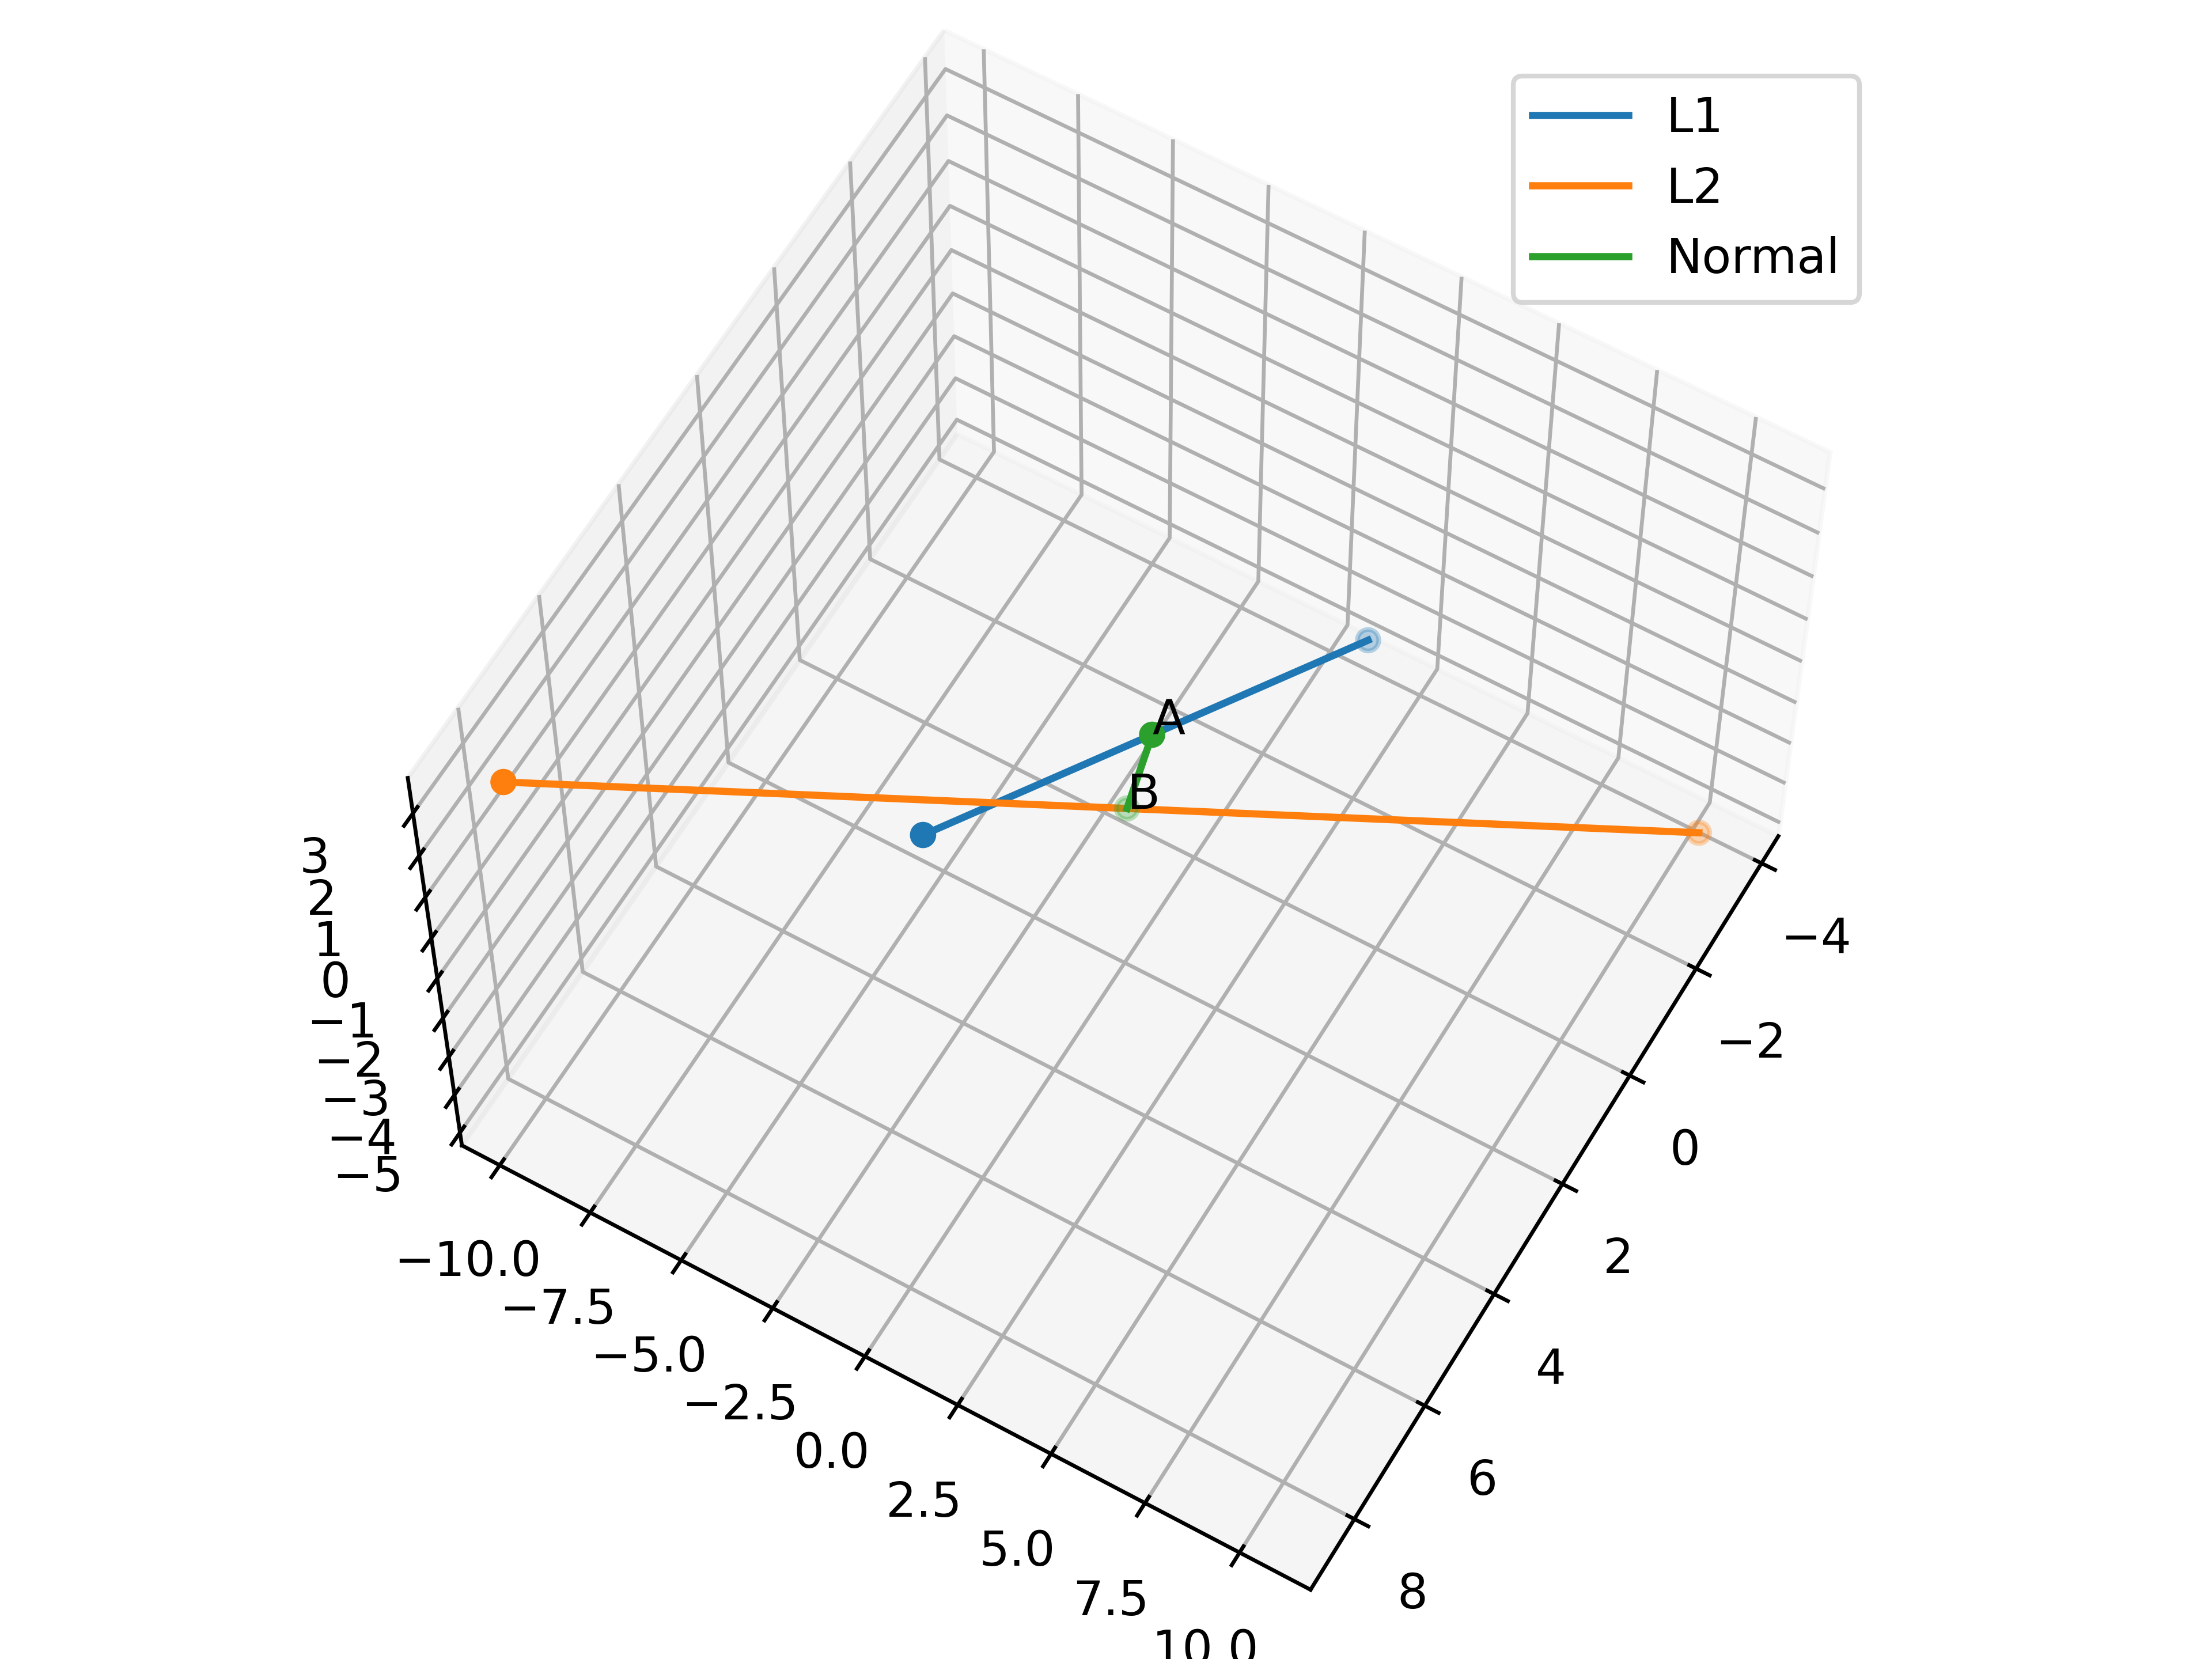
\includegraphics[width=\columnwidth]{chapters/12/11/2/e11/figs/skew.png}
\caption{}
	\label{fig:chapters/12/11/2/e11/}
\end{figure}

\end{enumerate}

